\documentclass{article}

\usepackage{arxiv}

\usepackage[spanish]{babel}
\usepackage[utf8]{inputenc} % allow utf-8 input
\usepackage[T1]{fontenc}    % use 8-bit T1 fonts
\usepackage{hyperref}       % hyperlinks
\usepackage{cleveref}       % clever references (\cref)
\usepackage{url}            % simple URL typesetting
\usepackage{booktabs}       % professional-quality tables
\usepackage{amsfonts}       % blackboard math symbols
\usepackage{nicefrac}       % compact symbols for 1/2, etc.
\usepackage{microtype}      % microtypography
\usepackage{lipsum}
\usepackage{graphicx}
\usepackage{float}
\graphicspath{{./images/}{./images/graficos/}}


\title{TP 1.2 - ESTUDIO ECONÓMICO-MATEMÁTICO DE APUESTAS EN LA RULETA}


\author{
    Alvaro Tomasino \\
    Ingeniería en Sistemas de Información\\
    Universidad Tecnológica Nacional - FRRO\\
    Zeballos 1341, S2000, Argentina\\
    \texttt{atomasino08@gmail.com} \\
\And
    Melina Aronson \\
    Ingeniería en Sistemas de Información\\
    Universidad Tecnológica Nacional - FRRO\\
    Zeballos 1341, S2000, Argentina\\
    \texttt{melinaaronson@gmail.com} \\
\And
    Tomas Aguilera \\
    Ingeniería en Sistemas de Información\\
    Universidad Tecnológica Nacional - FRRO\\
    Zeballos 1341, S2000, Argentina\\
    \texttt{tomas.aguilera.27@gmail.com} \\
\And
    Juan Bautista Martinelli \\
    Ingeniería en Sistemas de Información\\
    Universidad Tecnológica Nacional - FRRO\\
    Zeballos 1341, S2000, Argentina\\
    \texttt{martinellij4@gmail.com} \\
}




\begin{document}

\maketitle




\begin{abstract}
  El siguiente documento tiene por objetivo detallar el trabajo de investigación que debe realizarse para profundizar el estudio del comportamiento de la ruleta pero desde el punto de vista del apostador y sus estrategias.
\end{abstract}

\keywords{Simulación \and Trabajo práctico \and Ruleta \and apuestas \and estrategias}






\section{Introducción}
En el trabajo anterior (TP 1.1), se modeló el funcionamiento de la ruleta europea, validando su comportamiento con la distribución uniforme discreta, la Ley de los Grandes Números y el Teorema Central del Límite, a través de la estabilización de estadísticos como el valor promedio y la varianza.

El objetivo de este trabajo es profundizar esta investigación, cambiando el foco desde el funcionamiento de la ruleta hacia un análisis económico-matemático desde la perspectiva del apostador. El propósito es desmitificar estadísticamente la verdadera probabilidad de obtener ganancias sostenibles usando distintas estrategias de apuestas en un medio ideal simulado.

Para alcanzar este objetivo, se analizan cuatro estrategias: Martingala, D'Alembert, Fibonacci y Paroli. Cada estrategia se somete a dos supuestos mutuamente excluyentes:

\begin{itemize}
  \item \textbf{Capital acotado (finito):} un escenario realista donde se analiza la probabilidad de bancarrota y el impacto de los límites financieros sobre la viabilidad de la estrategia a largo plazo.
  \item \textbf{Capital infinito:} un escenario ideal que permite observar el comportamiento matemático teórico de la estrategia sin restricciones de fondos.
\end{itemize}

A través de esta simulación, se busca obtener una visión objetiva de la viabilidad de las apuestas, usando herramientas de visualización de datos para contrastar los resultados empíricos con las expectativas teóricas del apostador.

Las estrategias pueden ser de dos enfoques distintos:

\paragraph{Estrategias de progresión negativa} Se basan en aumentar la apuesta después de cada pérdida, buscando recuperar el capital cedido en una sola tirada ganadora. La desventaja es que es riesgoso, porque una racha negativa prolongada puede agotar rápido el capital.

\paragraph{Estrategias de progresión positiva} Se basan en aumentar la apuesta después de cada acierto, buscando capitalizar las rachas ganadoras. Este enfoque se considera más conservador, porque busca maximizar los beneficios usando el dinero ganado al casino en vez de “perseguir pérdidas” con el capital base.




\section{Metodología}
\label{sec:metodologia}

\subsection{Diseño del modelo}
A diferencia del modelo anterior, que se centraba en la frecuencia de aparición de números, este modelo incorpora una lógica de gestión de banca (bankroll) y flujo de caja (cash flow). El sistema procesa los siguientes parámetros de entrada por consola:

\begin{itemize}
  \item \texttt{-c} (corridas): cantidad de simulaciones independientes.
  \item \texttt{-n} (muestras): cantidad de tiradas por corrida.
  \item \texttt{-s} (estrategia): estrategia utilizada, que puede ser martingala (m), D’Alembert (d), Fibonacci (f) o Paroli (o).
  \item \texttt{-a} (capital): tipo de capital, que puede ser infinito (i) o finito (f).
\end{itemize}

\subsection{Procesamiento de datos}
En esta segunda etapa de la investigación, el análisis se deja de enfocar en números individuales y pasa a enfocarse en eventos de “éxito o fracaso”. Para modelar esto, se usó la \textbf{Distribución Binomial} ($X\sim \mathrm{Bi}(n,p)$), que es adecuada para representar las estrategias de apuestas elegidas (Martingala, D’Alembert, Fibonacci y Paroli) aplicadas a “apuestas simples”.

Cada tirada de la ruleta se considera un \textbf{ensayo de Bernoulli} independiente, donde solo hay 2 resultados posibles: éxito (ganar la apuesta) o fracaso (perder la apuesta). Como ejemplo, tomamos como “éxito” que el número obtenido sea par (sin contar el 0), lo que define los parámetros de la distribución:

\begin{itemize}
  \item \textbf{n (ensayos)}: es la cantidad de tiradas realizadas en cada corrida de la simulación.
  \item \textbf{p (probabilidad de éxito)}: se calcula dividiendo la cantidad de números favorables (18 números pares) por el total de números de la ruleta europea (37): $p = 18/37 \approx 0.486$.
\end{itemize}

Para comparar los resultados obtenidos con los valores teóricos, el sistema calcula los estadísticos de referencia:

\begin{itemize}
  \item \textbf{Frecuencia relativa esperada (fr\_e)}: representa la probabilidad teórica de éxito en cada ensayo (p). En el código se define como \texttt{len(par)/cant\_numeros\_ruleta}.
  \item \textbf{Valor promedio esperado (vp\_e)}: representa la media de la distribución binomial y se calcula multiplicando la cantidad de tiradas por la probabilidad de éxito. En el código se calcula como \texttt{tiradas*fr\_e}.
\end{itemize}

Este marco estadístico permite analizar el rendimiento económico del apostador, comparando los beneficios obtenidos en la simulación con la ventaja matemática que tiene el casino.




\subsection{Implementación de estrategias de apuestas}



\subsubsection{Martingala}
La Martingala es una estrategia de \textbf{progresión negativa}. Proporciona al jugador una alta probabilidad de ganar muchas pequeñas cantidades, a cambio de un bajo riesgo de perder mucho. Se basa en apuestas simples, que son las que tienen una probabilidad de ganar o perder cercana al 50\% (como apuestas par/impar, o rojo/negro).

\paragraph{Funcionamiento} Consiste en duplicar la apuesta después de cada pérdida. El objetivo es que, si el jugador gana, recupere todas las pérdidas acumuladas en las rondas anteriores más un beneficio adicional equivalente a la apuesta inicial.

\paragraph{En la simulación} El ciclo empieza con una apuesta base (\texttt{apuesta\_martingala = 1}). Si se gana (\texttt{valores[nro\_tirada] in par}), el capital aumenta, se agrega el beneficio al flujo de caja y la apuesta se reinicia al valor base. Si se pierde, se resta la apuesta del capital actual y se duplica el monto para la siguiente tirada (\texttt{apuesta\_martingala *= 2}). En el escenario de capital acotado (\texttt{tipo\_capital == 'f'}), se activa la condición de bancarrota si el capital es negativo o si el monto de la apuesta necesaria supera el dinero disponible del apostador.

\subsubsection{D’Alembert}
D’Alembert es otra estrategia de \textbf{progresión negativa}, y también se basa en apuestas simples. Se basa en la idea de que dos resultados de igual probabilidad ocurren con la misma frecuencia, por lo que las probabilidades de éxito son mayores cuanto más dinero se tenga para apostar. Pero esto también implica que se puede perder más.

\paragraph{Funcionamiento} El jugador usa una secuencia de 10 números, que representa una unidad de apuesta. El monto a apostar se determina sumando el primer y el último número de esa secuencia. Si se gana la apuesta, esos números se tachan. Si se pierde, se agrega el monto fallido al final de la secuencia para intentar recuperarlo en la siguiente ronda. El objetivo es haber ganado 10 unidades una vez que se hayan tachado todos los números.

\paragraph{En la simulación} Se inicializa una lista con la secuencia base de unidades (\texttt{arr\_dalembert = [1,1,1,1,1,1,1,1,1,1]}). La apuesta actual se calcula sumando el primer y último elemento de esa secuencia (\texttt{arr\_dalembert[0] + arr\_dalembert[-1]}). Si se gana, se eliminan los dos extremos de la lista (\texttt{arr\_dalembert.pop(0)} y \texttt{arr\_dalembert.pop(-1)}). Si se pierde, el monto de la apuesta fallida se agrega al final de la secuencia (\texttt{arr\_dalembert.append(apuesta)}). La bancarrota se verifica comparando si la suma de los extremos necesaria para la siguiente jugada excede el capital disponible en \texttt{dinero\_dalembert\_corrida}.

\subsubsection{Fibonacci}
Fibonacci es otra estrategia de \textbf{progresión negativa}, y también se basa en apuestas simples. Está basada en la secuencia matemática de números donde cada número es igual a la suma de los dos anteriores ($1, 1, 2, 3, 5, 8, 13, 21$ y así sucesivamente).

\paragraph{Funcionamiento} Se tiene una secuencia de números para establecer las unidades que se apuestan. Una unidad es la cantidad que se apuesta en cada mano. Si se pierde, se avanza un nivel en la secuencia para establecer la siguiente unidad de apuesta. Si se gana, se retroceden 2 posiciones, permitiendo recuperar pérdidas acumuladas sin disparar el monto apostado de forma exponencial.

\paragraph{En la simulación} Se genera la secuencia matemática en la lista \texttt{s\_fibonacci} y se usa un puntero (\texttt{posicion\_secuencia}) para determinar el monto a apostar. Si se gana, se retroceden dos posiciones en la secuencia (\texttt{max(posicion\_secuencia - 2, 0)}). Si se pierde, se avanza una posición hacia la derecha (\texttt{posicion\_secuencia + 1}). El estado de bancarrota se alcanza si el valor de la secuencia correspondiente a la posición actual es mayor al capital restante del jugador en la corrida.

\subsubsection{Paroli}
Paroli es una estrategia de \textbf{progresión positiva}. Se basa en la idea de que ganancias y pérdidas suelen ocurrir por rachas, por lo que buscar maximizar el beneficio apostando más en las rachas ganadoras y menos en las rachas perdedoras.

\paragraph{Funcionamiento} El objetivo es ganar 3 veces consecutivas, doblando la apuesta después de cada victoria. Se empieza apostando una sola unidad. Si se gana, la apuesta se duplica. Si se pierde, se vuelve a apostar una sola unidad, asegurando que nunca se arriesgue más de una unidad del presupuesto base por ciclo.

Aunque cada progresión Paroli termina en una pérdida o en 3 ganancias consecutivas, es bueno dividir la jugada en grupos de 3 apuestas para entender los posibles resultados:

\begin{figure}[H]
  \centering
  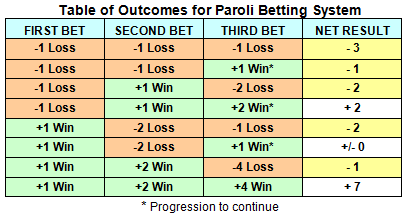
\includegraphics[width=0.6\textwidth]{tabla-paroli.png}
  \caption{Tabla de progresión Paroli.}
\end{figure}

\paragraph{En la simulación} Se usa una unidad base (\texttt{apuesta\_paroli = 1}) y un contador de rachas (\texttt{acumulador\_ganancias\_seguidas}). Si se gana, la apuesta se duplica (\texttt{apuesta\_paroli *= 2}) y el contador aumenta. Si se pierde o si se gana 3 veces consecutivas, la apuesta se reinicia a 1 unidad y el contador vuelve a cero. El sistema comprueba la bancarrota comparando la apuesta reiniciada o duplicada contra el flujo de caja final de la tirada (\texttt{dinero\_paroli\_corrida[-1]}).





\section{Resultados}
\label{sec:resultados}

\subsection{Gráficos de los resultados}
Para graficar los resultados de la simulación, usamos el paquete \texttt{Matplotlib}, analizando cada estrategia en distintos contextos.

Considerando un capital \textbf{finito}, se muestran 3 gráficos por estrategia: la evolución del flujo de caja en una sola corrida (\texttt{plt.plot}), la dispersión del capital final después de 3000 corridas (\texttt{plt.scatter}) y el rendimiento promedio obtenido frente al capital inicial (\texttt{plt.bar}).

Cada gráfico se muestra comparando la cantidad de tiradas entre $n=100$ y $n=1000$, demostrando que mientras más se juega, más se degrada el capital y la probabilidad de bancarrota aumenta.

Considerando un capital \textbf{infinito}, se muestran 2 gráficos por estrategia: uno de ganancia acumulada vs pérdida acumulada y uno del saldo neto.

\subsubsection{Estrategia Martingala}


\paragraph{Flujo de caja (1ra corrida)} En el primer gráfico (con 100 tiradas), se observa una serie de tiradas donde el capital fluctúa cerca del valor inicial de \$100 antes de una caída abrupta hacia la bancarrota en la tirada 7. Al comparar con el segundo gráfico (con 1000 tiradas), se ve un periodo de supervivencia más extenso, pero con una pendiente de caída final mucho más pronunciada hacia la tirada 19, evidenciando el riesgo del crecimiento exponencial de la apuesta.

\paragraph{Dispersión de capital final} El primer gráfico (con 100 tiradas) muestra una concentración de resultados finales entre \$140 y \$160, con una franja significativa de bancarrotas cerca de cero. En el segundo gráfico (con 1000 tiradas), la cantidad de puntos abajo del capital inicial es mucho más densa, confirmando una mayor frecuencia de fallos acumulados a largo plazo.

\paragraph{Rendimiento promedio} El primer gráfico (con 100 tiradas) muestra un promedio final de \$92,43, que es una pérdida moderada respecto al capital inicial. En el segundo gráfico (con 1000 tiradas), el promedio cae drásticamente a \$76,15, validando que cuanto más se juega, más se pierde.

\paragraph{Análisis con capital infinito} Los gráficos demuestran la progresión negativa. La línea de ganancia acumulada se mantiene por encima de la pérdida y, aunque hay una caída crítica, el sistema se recupera en la siguiente tirada exitosa. Al final, el saldo neto es positivo, demostrando que sin límites de capital la Martingala puede generar un beneficio temporal.

\subsubsection{Estrategia Fibonacci}
\paragraph{Flujo de caja (1ra corrida)} El primer gráfico (con 100 tiradas) muestra una volatilidad controlada, donde el flujo de caja se recupera parcialmente retrocediendo 2 posiciones en la secuencia después de cada acierto. En el segundo gráfico (con 1000 tiradas), la racha negativa prolongada termina superando la capacidad de recuperación, resultando en bancarrota en la tirada 40.

\paragraph{Dispersión de capital final} En el primer gráfico (con 100 tiradas), los resultados finales están más dispersos, con bastantes casos por arriba de la línea del capital inicial. En cambio, el segundo gráfico (con 1000 tiradas) muestra cómo la mayoría de las corridas terminan con un capital residual mínimo, agotado por la progresión de la secuencia.

\paragraph{Rendimiento promedio} En el primer gráfico (con 100 tiradas), se ve un capital promedio final de \$94,39. En el segundo gráfico (con 1000 tiradas), el rendimiento disminuye a \$72,07, demostrando que la progresión negativa de Fibonacci no compensa el margen de la casa en sesiones extensas.

\paragraph{Análisis con capital infinito} El crecimiento del capital es más escalonado que en la Martingala. La estrategia puede recuperarse de rachas negativas importantes gracias a retroceder 2 posiciones después de un acierto. Aunque la ganancia final es menor que en otras estrategias, el crecimiento se sostiene si no hay límites de capital.

\subsubsection{Estrategia D’Alembert}
\paragraph{Flujo de caja (1ra corrida)} El primer gráfico (con 100 tiradas) refleja una pérdida lineal constante hasta la bancarrota en la tirada 30. El segundo gráfico (con 1000 tiradas) muestra un comportamiento parecido, donde pequeñas recuperaciones no logran revertir la tendencia negativa, llegando a la bancarrota en la tirada 38.

\paragraph{Dispersión de capital final} El primer gráfico (con 100 tiradas) muestra resultados muy variados, con una gran cantidad de corridas terminando en saldo negativo. En el segundo gráfico (con 1000 tiradas), la dispersión se concentra casi exclusivamente en valores cercanos a cero o negativos.

\paragraph{Rendimiento promedio} En el primer gráfico (con 100 tiradas) muestra un promedio final de \$87,17. En el segundo gráfico (con 1000 tiradas), ese valor disminuye a \$51,15, siendo la caída más agresiva entre las estrategias analizadas.

\paragraph{Análisis con capital infinito} El primer gráfico muestra aumentos importantes después de rachas de fallos, por lo que el segundo gráfico tiene una recuperación constante gracias a la naturaleza aritmética de sumar los dos extremos. Al final, se logra un saldo neto positivo si no hay límites de capital.

\subsubsection{Estrategia Paroli}
\paragraph{Flujo de caja (1ra corrida)} Al ser una progresión positiva, el primer gráfico (con 100 tiradas) muestra picos de ganancia cuando se encadenan aciertos, pero sin caídas exponenciales ante pérdidas. El segundo gráfico (con 1000 tiradas) muestra que, aunque se logren picos de hasta \$250, la varianza estadística termina erosionando el capital inicial a largo plazo.

\paragraph{Dispersión de capital final} El primer gráfico (con 100 tiradas) muestra la cantidad de puntos muy equilibrada alrededor de la línea de capital inicial, con pocas bancarrotas inmediatas. En el segundo gráfico (con 1000 tiradas), aunque hay valores altos, se ve una línea densa de corridas en \$0, demostrando que incluso con bajo riesgo por apuesta, el tiempo de juego agota el capital.

\paragraph{Rendimiento promedio} En el primer gráfico (con 100 tiradas), el capital promedio final es de \$95,89, el más alto de las 4 estrategias para $n=100$. Pero en el segundo gráfico (con 1000 tiradas), el promedio cae a \$57,89, reforzando que ninguna estrategia supera la ventaja matemática del casino al aumentar la cantidad de ensayos.

\paragraph{Análisis con capital infinito} Al no aumentar las apuestas tras una pérdida, Paroli depende de rachas ganadoras para recuperar pérdidas, por lo que su rendimiento final es más incierto. Los gráficos muestran variaciones alrededor del punto de equilibrio, aunque pueden existir picos positivos temporales.

\subsubsection{Convergencia del porcentaje de victorias}
El gráfico de convergencia muestra cómo, a medida que aumenta la cantidad de tiradas, el porcentaje observado de victorias tiende a estabilizarse en el 48,6\% teórico (18/37). Esta estabilización confirma la Ley de los Grandes Números en eventos binarios, proporcionando un marco sólido para comparar los resultados de las estrategias frente al valor esperado.

\subsection{Comparación de rendimientos por estrategia}
Para analizar cómo influye la cantidad de tiradas en el resultado económico de cada estrategia, comparamos el capital promedio final obtenido después de 3000 corridas. Así, se puede ver cómo evoluciona el capital inicial de \$100 frente a la ventaja matemática del casino.

\begin{table}[H]
  \centering
  \begin{tabular}{lcccc}
    \toprule
    Estrategia & Capital prom final (n=100) & \% bancarrota & Capital prom final (n=1000) & \% bancarrota \\
    \midrule
    Martingala & \$92,43 & 14,2\% & \$76,15 & 84,7\% \\
    Fibonacci  & \$94,39 & 9,8\% & \$72,07 & 89,1\% \\
    D’Alembert & \$87,17 & 18,5\% & \$51,15 & 94,3\% \\
    Paroli     & \$95,89 & 4,1\% & \$57,89 & 79,6\% \\
    \bottomrule
  \end{tabular}
  \caption{Comparación de rendimientos finales según la cantidad de tiradas}
\end{table}

Como se ve en la tabla, ninguna de las estrategias pudo mantener el capital inicial de \$100.

A \textbf{corto plazo (n=100)}, Paroli obtuvo el mejor resultado promedio, por ser una estrategia de progresión positiva, donde las apuestas aumentan después de ganar y no después de perder.

A \textbf{largo plazo (n=1000)}, todas muestran pérdidas mucho más marcadas. La estrategia D’Alembert fue la que más cayó respecto al capital inicial.

Esto confirma que, aunque algunas estrategias pueden parecer exitosas en pocas tiradas, la \textbf{Ley de los Grandes Números} garantiza que el flujo de caja del apostador tienda inevitablemente hacia la pérdida a medida que aumenta el número de ensayos de Bernoulli.


\section{Discusión}
Los resultados obtenidos permiten hacer un análisis más realista de la viabilidad de las estrategias de apuestas. El gráfico de convergencia de victorias (que estabiliza el éxito en el 48,6%) demuestra que los ensayos de Bernoulli representan una ruleta europea ideal, sin sesgos físicos.

Al analizar el impacto de aumentar la cantidad de tiradas, la tabla 1 demuestra la Ley de los Grandes Números. En sesiones de juego cortas (n=100), el capital promedio final se mantiene relativamente cerca del inicial. La estrategia Paroli (de progresión positiva) mostró el mejor desempeño, con la menor tasa de bancarrota. Esto muestra que, a corto plazo, la variabilidad del azar puede favorecer al jugador, o permitirle conservar gran parte de su capital.

Pero cuando la cantidad de tiradas aumenta (n=1000), todas las estrategias muestran una degradación del capital y un aumento en la tasa de bancarrota, mucho más marcado.

Los supuestos de capital infinito y finito muestran la diferencia entre la teoría y la práctica. Con un capital infinito, las estrategias de progresión negativa (Martingala, Fibonacci y D’Alembert) parecen efectivas desde un punto de vista matemático ideal, porque eventualmente recuperan pérdidas después de una racha negativa. Pero en la práctica, con un capital acotado, esta misma lógica acelera la quiebra.

Los resultados obtenidos muestran que no existen estrategias “ganadoras”. Las estrategias no alteran la probabilidad de éxito de cada tirada, sino que solo cambian la forma en que se distribuyen las ganancias y pérdidas en el tiempo. La ventaja matemática del casino del 2,7% (generada por el 0) termina apareciendo inevitablemente cuando aumenta la cantidad de tiradas.


\section{Conclusiones}
Este trabajo permitió modelar y analizar el comportamiento económico de distintas estrategias de apuestas con una simulación en Python. A través del análisis del flujo de caja, las ganancias, pérdidas y situaciones de bancarrota, se logró desmitificar estadísticamente la probabilidad de obtener ganancias sostenibles en la ruleta.

Con los resultados obtenidos, se llegó a la conclusión de que ninguna de las estrategias analizadas logra superar la esperanza matemática negativa del juego a largo plazo.

Las estrategias de progresión negativa (Martingala, D’Alembert y Fibonacci) presentan un riesgo alto en escenarios reales de capital finito, porque una racha moderada de pérdidas obliga a hacer apuestas que superan rápidamente el capital del jugador.

La estrategia de progresión positiva (Paroli) fue la más resistente a la bancarrota inmediata, al arriesgar principalmente las ganancias acumuladas. Pero incluso esta estrategia termina con pérdidas cuando la cantidad de tiradas es suficientemente grande.

La simulación permitió comprobar experimentalmente la Ley de los Grandes Números. Cuanto mayor es la cantidad de tiradas, los resultados observados se aproximan cada vez más a la pérdida esperada, por lo que la única variable que puede controlar el apostador es su tiempo de permanencia jugando.

Todo esto refuerza la idea de que la ruleta es un sistema de azar diseñado con una ventaja matemática favorable al casino. Las distintas estrategias pueden modificar la variabilidad de los resultados o retrasar las pérdidas, pero no cambian las probabilidades del juego.


\nocite{*}

\bibliographystyle{unsrturl}
\bibliography{references}

\end{document}


